\chapter{Electronics}

\section{Trigger Hub}
\label{app:electronics:trigger_hub}

The trigger hub is driven by a \SI{3.3}{\volt} input signal and a
\SI{5}{\volt} voltage source. The input signal is amplified to drive four
\gls{ttl} inputs through use of the \gls{sn74128} \cite{SN74128} line driver.
Furthermore the hub is designed to be mounted on the \gls{bbb} which itself
provides the trigger network interface.

\begin{figure}[h]
  \centering
  \captionsetup{width=.8\textwidth}
  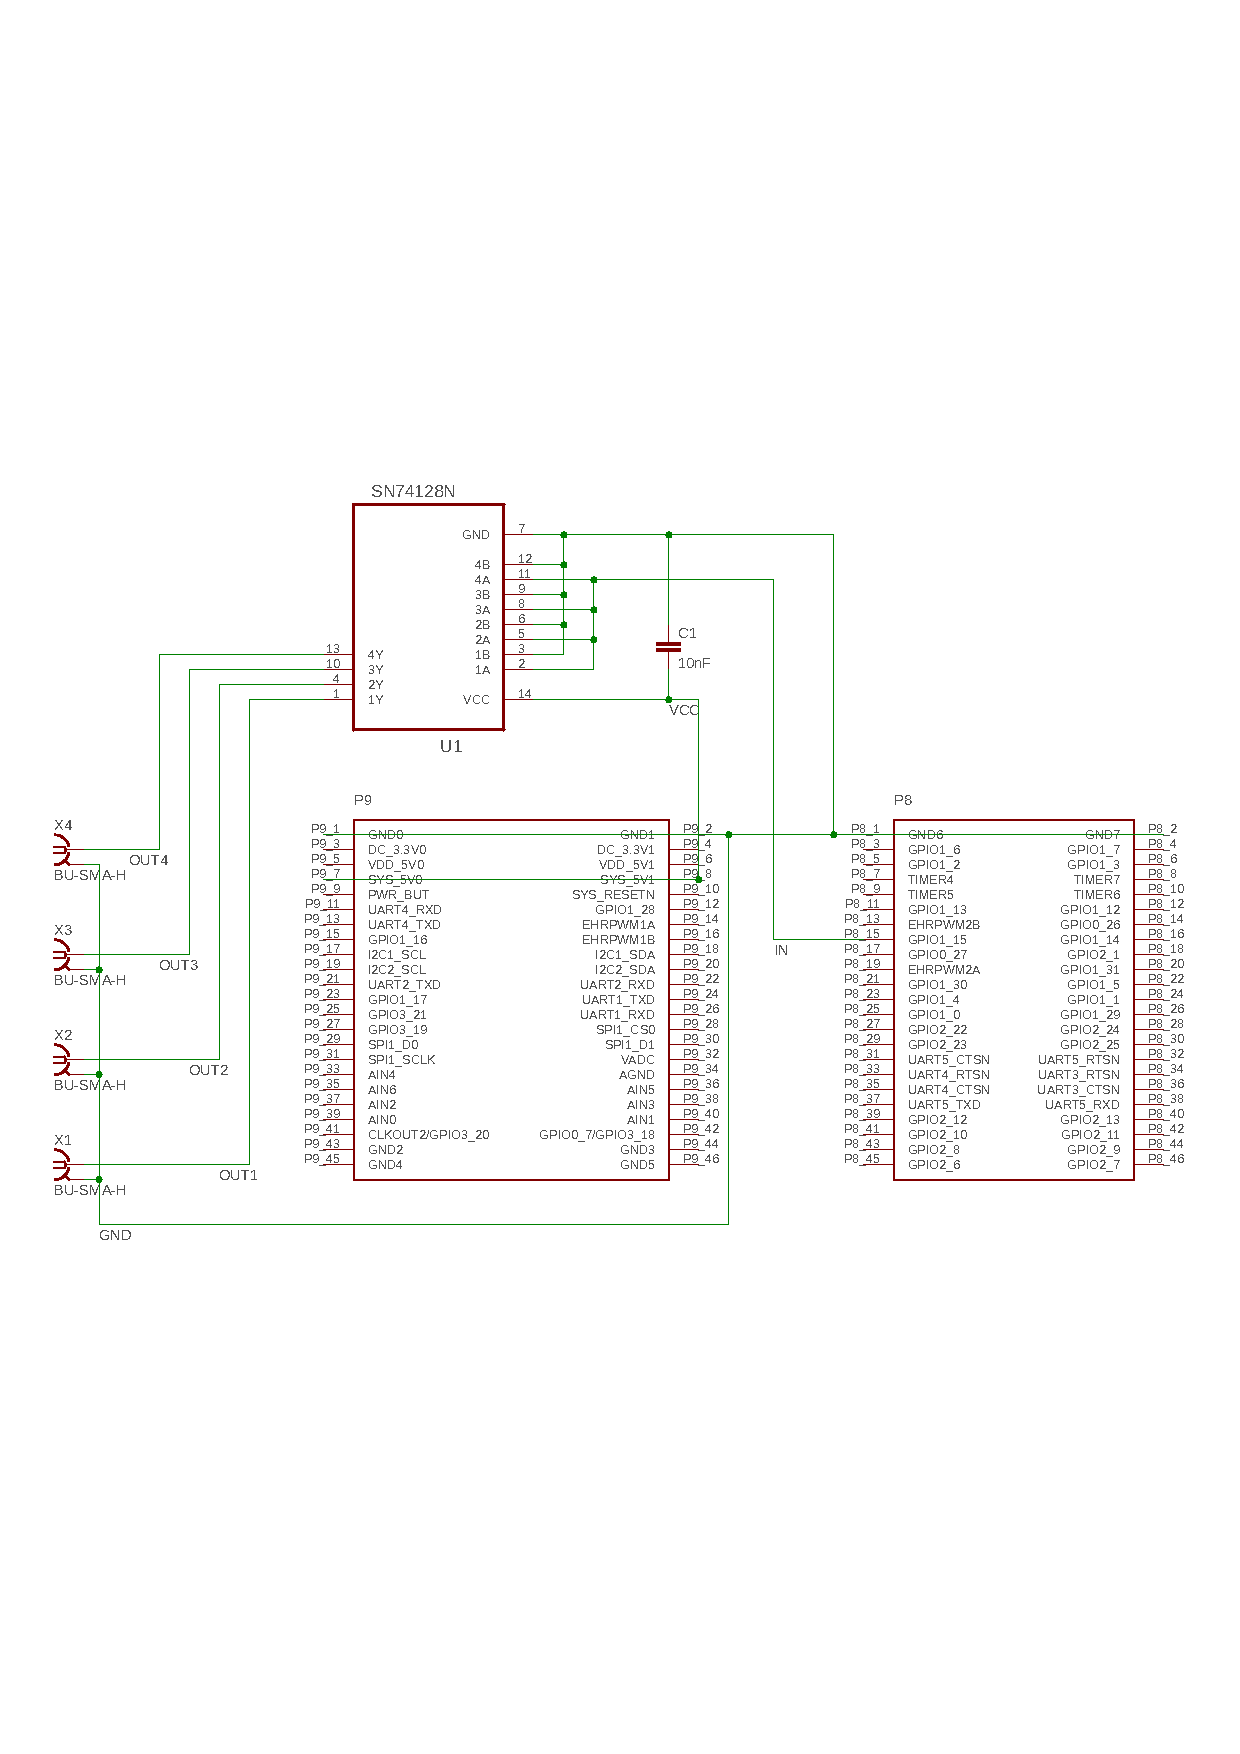
\includegraphics[width=\textwidth]{images/circuits/line-driver/schematic.pdf}
  \caption{Elecronic circuit schematics of the trigger hub. The
    \SI{3.3}{\volt} input signal is amplified by the \gls{sn74128} line
    driver and outputed to four \gls{sma} connectors.}
\end{figure}

The \gls{sn74128} exposes four independent outputs $Y$, each is driven by a
two-input ($A$ and $B$) with NOR ($\overline{A+B}=Y$) logic. As our objective
is to forward rising edge trigger signals we pulled all four $B$ to low by
connecting them with \gls{gnd}. The four $A$ where connected together with
the input signal. The input signal has to transition from $1$ to $0$ in order
to signal a rising edge trigger signal.

\begin{listing}[h]
  \inputminted[xleftmargin=.2\linewidth]{javascript}{scripts/trigger.js}
  \captionsetup{width=.6\linewidth}
  \caption{\gls{bbb} script that starts a \gls{http} server to listen for
requests on which to trigger a rising edge signal. On execution it pulls the
signal \gls{gpio} to high. The request callback then pulls the \gls{gpio} to
low for one \SI{1}{\milli\second}.}
\end{listing}

Using the \gls{bbb} makes it easy to write scripts that communicate with
other devices over the \gls{lan}. We used the bonescript library to access
the \gls{gpio} interface as it is pre-installed on the \gls{bbb}.
